% Generated assets: experiments/create_feature_ablation_plots.py.
% Legacy asset filenames are retained; the quantities are feature ablations.
\begin{figure}[htbp]
\centering
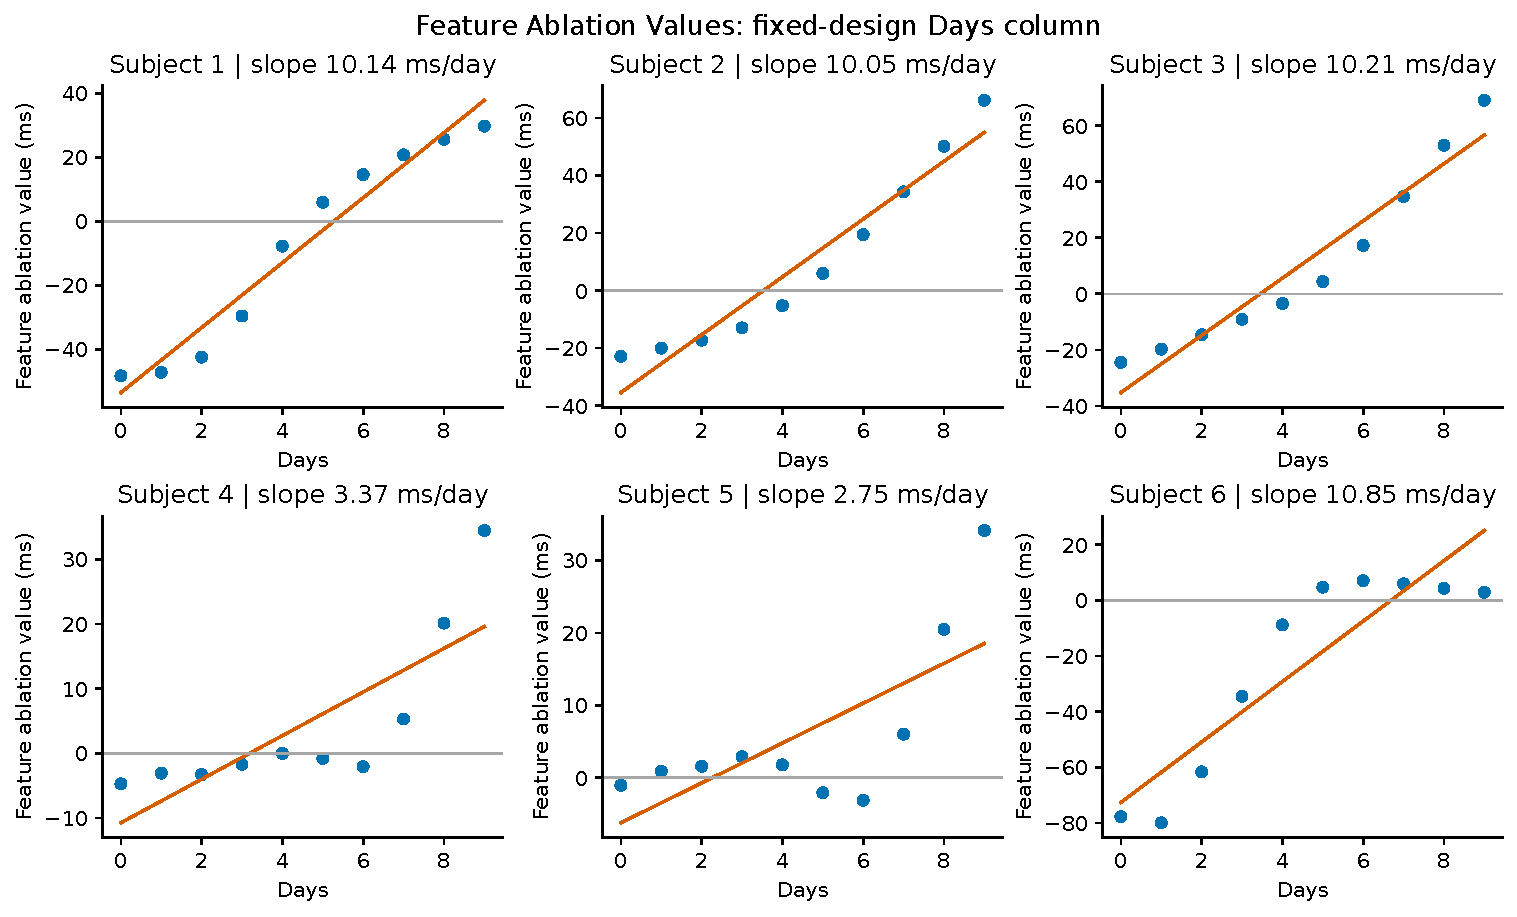
\includegraphics[width=\textwidth]{shap_days_effect_per_subject.pdf}
\caption{Fixed-design Days ablation values for six subjects, in milliseconds. Each point is the prediction minus its value after replacing the fixed-design Days column by the training-background mean, with the random-slope inputs and group indices held fixed. Lines are descriptive least-squares summaries, with slopes in ms/day. This is a full-data illustration, not held-out prediction assessment or recovery of subject-specific random coefficients. Subjects have anonymous source-order labels.}
\label{fig:ablation_days_effects}
\end{figure}

\begin{figure}[htbp]
\centering
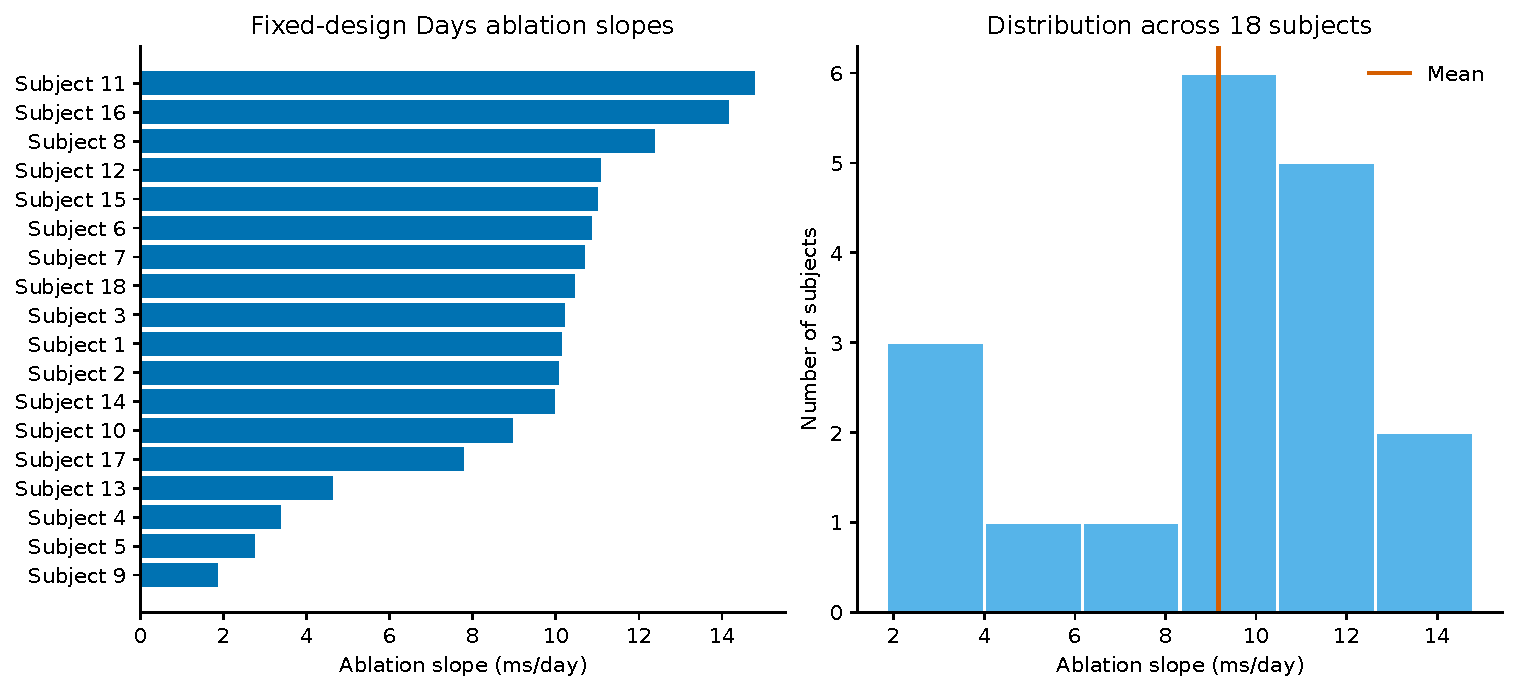
\includegraphics[width=\textwidth]{shap_subject_effect_comparison.pdf}
\caption{Ablation slopes from the fixed-design Days perturbation across all 18 subjects. Left: ordered descriptive line slopes in ms/day. Right: their distribution, with a line marking the mean. These summaries describe the fitted function under a specified perturbation; they do not estimate the random-slope variance component.}
\label{fig:ablation_subject_comparison}
\end{figure}

\begin{figure}[htbp]
\centering
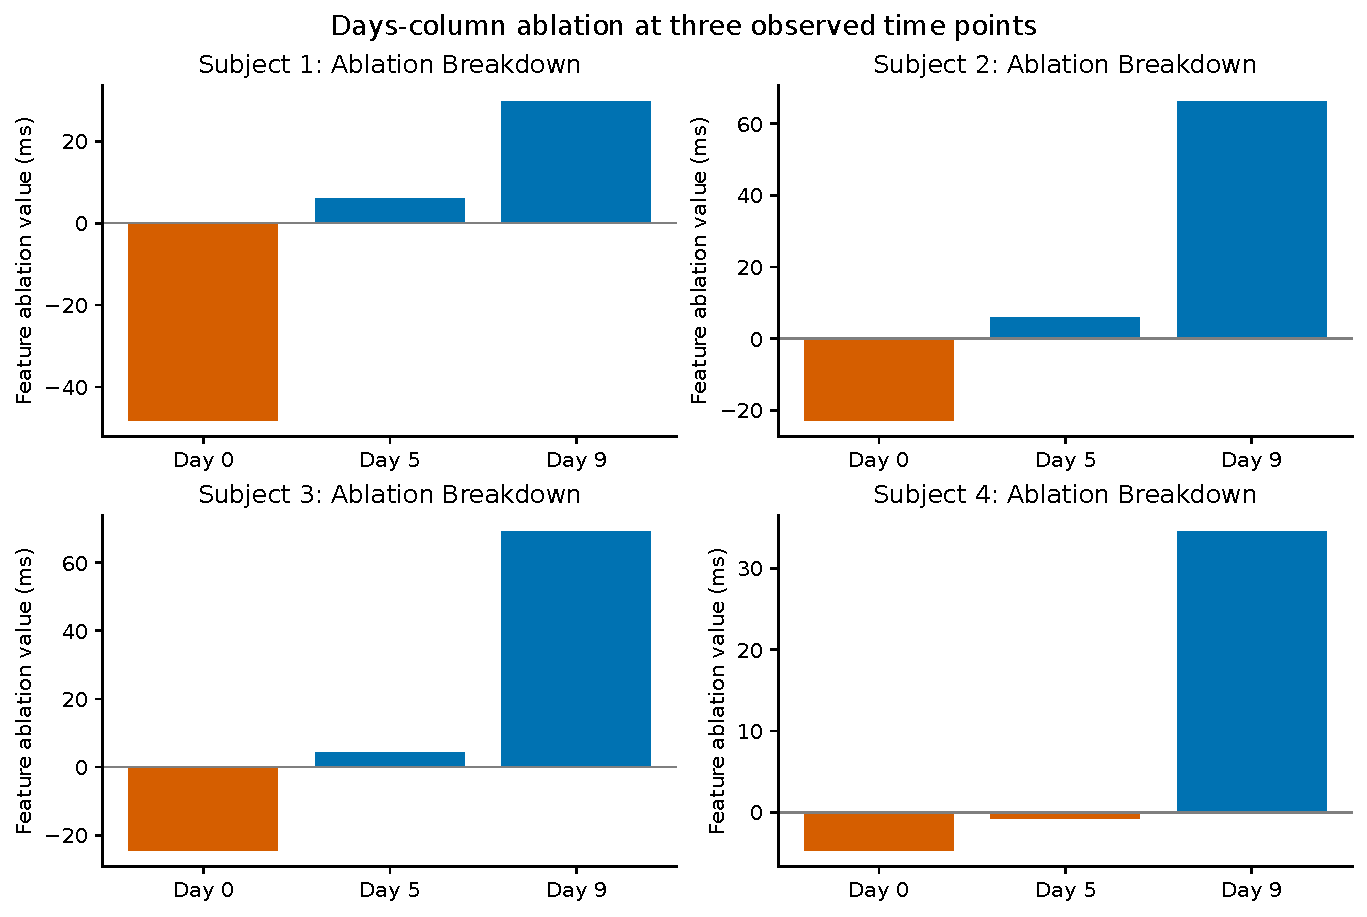
\includegraphics[width=0.95\textwidth]{shap_waterfall_subjects.pdf}
\caption{Ablation breakdown for four subjects at observed Days 0, 5 and 9. Bars show the single fixed-design Days-column prediction difference in milliseconds, using the same background and frozen random-slope inputs as Figure~\ref{fig:ablation_days_effects}. Bars describe separate observations and are not accumulated to reconstruct a prediction.}
\label{fig:ablation_breakdown}
\end{figure}
